\documentclass[12pt]{article}
\usepackage[spanish, es-tabla]{babel}
\usepackage{amssymb, amsmath}
\usepackage{graphicx}
\usepackage[export]{adjustbox}
\title{Matemáticas para las Ciencias Aplicadas \\ Tarea 1}
\date{}
\author{Garcia Islas Fernando \\ Leo\\Mariana}
\begin{document}
\maketitle
\section{\large Un cohete}
Un cohete es disparado verticalmente hacia arriba y el combustible que lo impulsa se quema durante 60 segundos. Se sabe que, a los $h$ s de haber iniciado su desplazamiento, la altura $h$ (en metros) a la que se encuentra el cohete es: \[h(t) = 40 t^2 \; m\]
\begin{enumerate}

%Punto 1 del ejercicio 1
\item ¿A qué altura se halla el cohete cuando se le agota el combustible?
  
  \begin{align*}
    h(t)= 40t^2 \; \text{m} \hspace{5.1cm}    h(t)&=40(60)^2 \; m\\
t=60\text{s} \hspace{7cm}    &=40(3600) \; m\\
    &=144,000 \; m\\
  \end{align*}
  
  {\bf R:} 144,000 m es la altura cuando se agota el combustible.
  
  %Punto 2 del ejercicio 1
\item ¿Cuál es la rapidez promedio del cohete durante los primeros 60 s de su vuelo?
  
  \begin{align*}
    &\text{Rapidez promedio}=\frac{d}{t} \hspace{3cm}\frac{144,000}{60}= 2400 \frac{m}{s}\\
    &t = 60\; \text{s} \\
    &d = 40t^2 \; \text{m} 
  \end{align*}
  
  {\bf R:} $2,400 \frac{m}{s}$ es la rapidez promedio.
  
  %Punto 3 del ejercicio 1
\item Haga una tabla con tres columnas: una para el tiempo $t$ (donde $t = 0, 10, 20, . . . , 60 $s); otra para la posición $h(t)$; y una tercera para el incremento $\Delta h$ entre un valor de $t$ y el siguiente. Con base en ella, calcule la rapidez promedio del cohete para cada lapso de 10 s desde $t = 0$ hasta $t = 60$.
  
  \begin{table}[h]
  
    \begin{center}
  
        \begin{tabular}{| c | c | c |c|}\hline %Tabla 1
            $\Delta t$ s & $h(t)$ m & $\Delta h$ m&$\frac{h(t)}{t}\frac{m}{s}$\\ \hline
            0 & 0 & 0 &0 \\ 
            10& 4000& 4000& 4000 \\
            20&16,000&12,000&800\\
            30&36,000&20,000&1,200\\
            40&64,000&28,000&1,600\\
            50&100,000&36.000&2,000\\
            60& 144,000& 44,000& 2,400 \\ \hline
        \end{tabular}
    
    \caption{Rapidez promedio de intervalos $\Delta t$} 
    
    \label{tab:rapprom}
    
    \end{center}
  
  \end{table}

%Punto 4 del ejercicio 1
\item Haga ahora otra tabla en la que muestre el cálculo de la rapidez promedio del cohete $\Delta t$ s antes y $\Delta t$ s después de $t = 3$ s, para los siguientes valores de $\Delta t$:\[1,\frac{1}{10},\frac{1}{10^2},\frac{1}{10^3},\frac{1}{10^4},\frac{1}{10^5}.\]
  
    \begin{table}[h]
  
        \begin{center}
  
            \begin{minipage}{0.45\linewidth}
  
            \centering
  
                \begin{tabular}{| c | c | c |}\hline %Tabla 2
                  $\Delta t+3$  & $h(t)$  &$\frac{h}{t}$\\ \hline
                    4&640&160 \\
                    3.1&384.4&124\\
                    3.01&362.404&120.4\\
                    3.001&360.24004&120.04\\
                    3.0001&360.0240004&120.004\\
                    3.00001&360.0024&120.0004 \\ \hline
                \end{tabular}
            
            \caption{Rapidez promedio de intervalos $\Delta t + 3$}

            \label{tab:rapprom+3}

            \end{minipage}

            \hspace{0.05\linewidth} 

            \begin{minipage}{0.45\linewidth}

            \centering

            \begin{tabular}{| c | c | c |}\hline %Tabla 3
                $3 - \Delta t$  & $h(t)$  &$\frac{h}{t}$\\ \hline
                2&160&80 \\
                2.9&336.4&116\\
                2.99&357.604&119.6\\
                2.999&359.76004&119.96\\
                2.9999&359.9760004&119.996\\
                2.99999&359.9760004&119.9924\\ \hline
            \end{tabular}

            \caption{Rapidez promedio de intervalos $3 - \Delta t$}

            \label{tab:rapprom-3}

            \end{minipage}

        \end{center}

    \end{table}

%Punto 5 del ejercicio 1
\item Es razonable suponer que la rapidez instantánea del cohete exactamente a los $t = 3$ s, tomará un valor intermedio entre la rapidez promedio $\Delta t$ s antes y $\Delta t$ s después de $t = 3$. Si esto es cierto, según sus cálculos, ¿cuánto vale esa rapidez instantánea?\\
    
    {\bf R:} $120 \frac{m}{s}$, ya que el valor intermedio de la rapidez promedio de los valores $3- \Delta t$ y $\Delta t +3$ es cercano a 120.\par
    
%Punto 6 del ejercicio 1
\item Si la función $y = y(t)$ describe la posición de un objeto que se mueve con un solo grado de libertad, entonces la velocidad instantánea del móvil, $v = v(t)$, en cualquier instante $t$ de su desplazamiento se define como:
  
  \begin{equation}
    v(t) = \lim_{\Delta t \rightarrow \infty}\frac{y(t - \Delta t) - y(t)}{\Delta t}
  \end{equation}
  
  Aplique la definición (1) para mostrar que la velocidad del cohete, cuya posición para $0 \leq t \leq 60$ viene dada por $h(t) = 40t^2$, en el instante $t$ es $v(t) = 80t$. Calcule la velocidad exactamente a los $10$ s y los $45$ s de vuelo.
  
    \begin{align*}
        v(t) = \lim_{\Delta t \rightarrow \infty}\frac{h(t - \Delta t) - h(t)}{\Delta t}&= \lim_{\Delta t \rightarrow \infty}\frac{40(t - \Delta t)^2 - 40t^2}{\Delta t}\\
        &=\lim_{\Delta t \rightarrow \infty}\frac{40(t^2+2t\Delta t + \Delta t^2) - 40t^2}{\Delta t}\\
        &=\lim_{\Delta t \rightarrow \infty}\frac{40t^2+80t\Delta t + 40\Delta t^2 - 40t^2}{\Delta t}\\
        &=\lim_{\Delta t \rightarrow \infty}\frac{80t\Delta t + 40\Delta t^2}{\Delta t}\\
        &=\lim_{\Delta t \rightarrow \infty}\frac{\Delta t(80t+ 40\Delta)}{\Delta t}\\
        &=\lim_{\Delta t \rightarrow \infty}(80t+ 40\Delta) = 80t\\
    \end{align*}\\
    
    \begin{table}[h]
  
        \begin{center}
  
            \begin{tabular}{| c | c |}\hline %Tabla 4
                $t$ s & $v(t)$\\ \hline
                10 & 800 $\frac{m}{s}$\\ 
                45& 3,600 $\frac{m}{s}$  \\ \hline
            \end{tabular}
  
            \caption{Rapidez instantánea} 
  
            \label{tab:rapinst}
  
        \end{center}
  
    \end{table}
    
\end{enumerate}

\section{\large La pirámide del sol}

Según la Wikipedia, si se supone que la base de la pirámide del sol de Teotihuacan es cuadrada y que sus caras son lisas, su volumen es de $1.184828 \times 10^6 \, \text{m}^3$.

La versión en español de la misma enciclopedia informa que la altura de la pirámide es de $65$ m y el lado de su base mide $223$ m. A su vez, en la versión en inglés, se lee que la altura es de $71.17$ m y el lado de la base mide $223.48$ m. ¿Cuáles son los datos congruentes con el valor del volumen propuesto arriba si se sabe que el volumen $V$ de una pirámide viene dado por la fórmula:
    \[V = \frac{1}{3} A h \tag{2}\]

    donde $A$ es el área de la base y $h$, la altura?

    Si bien la fórmula (2) se puede obtener mediante argumentos geométricos relativamente simples en los que no se aplica el método de rebanar, aproximar y pasar al límite de Arquímedes (o de Eudoxo), este ejercicio tiene el propósito de experimentar numéricamente para encontrar una cota inferior y una cota superior del volumen $V$ de la pirámide del sol. Para ello, desarrolle los siguientes pasos:

\begin{enumerate}

%Punto 1 del ejercicio 2
    \item Imagine que hace 49 cortes transversales paralelos a la base, a intervalos regulares de altura $\Delta h = \frac{h}{50}$ donde $h$ es la altura de la pirámide (medida desde la cúspide hasta el centro de la base) y suponga que el volumen $V_j$ de la $j$-ésima rebanada es aproximadamente igual al:
  
        \begin{enumerate}
  
            \item Volumen del prisma circunscrito a la pirámide a la altura de esa $j$-ésima rebanada de altura $\Delta h$ para $j = 1, 2, \dots, 50$.
  
            \item Volumen del prisma inscrito a la pirámide a la altura de esa $j$-ésima rebanada de altura $\Delta h$ para $j = 0, 1, \dots, 49$.
  
        \end{enumerate}
  
        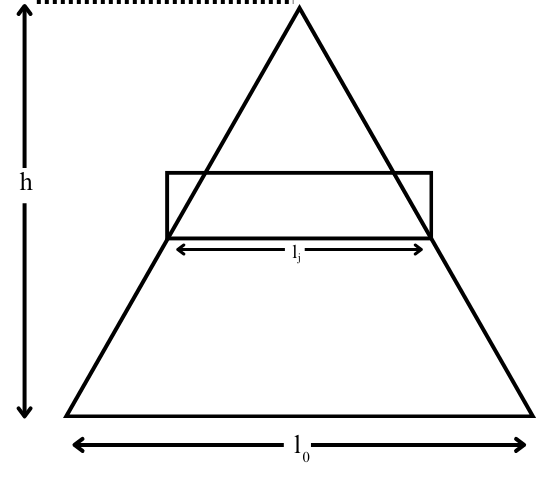
\includegraphics[width=0.5\textwidth, center]{piramide1.png}
  
        \[V_j = \Delta h \hspace{4.4pt}(l_j)^2\]

%Punto 2 del ejercicio 2
    \item Adapte el argumento que sugiere la siguiente figura (para el cálculo del volumen de un cono) al caso de la pirámide y aplíquelo para calcular los volúmenes $V_j$ de los prismas inscritos y circunscritos. 
 
        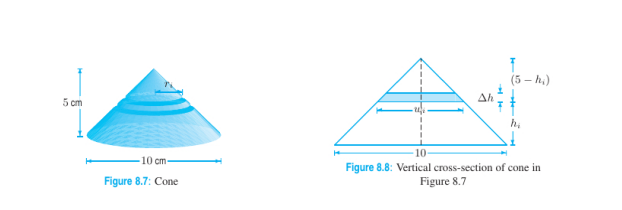
\includegraphics[width=0.5\textwidth, center]{cono.png} \\

        \begin{minipage}{0.4\textwidth}
            \raggedright
            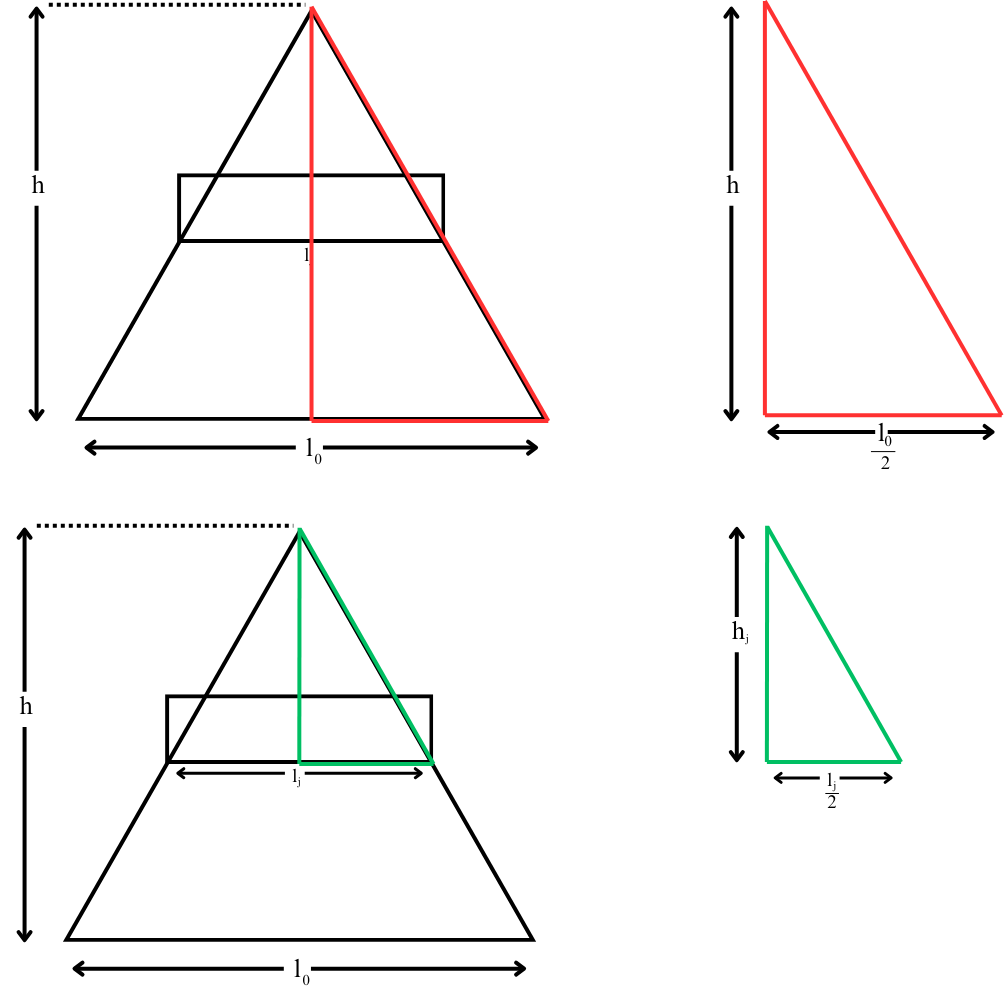
\includegraphics[width=\textwidth]{piramide2.png}
        \end{minipage}%
  
        \hfill
  
        \begin{minipage}{0.55\textwidth}
  
            \begin{align*}
                \Delta h &= \frac{h}{50}\\
                P &= \left\{ \frac{0h}{50}, \frac{1h}{50}, \frac{2h}{50}, \frac{3h}{50}, \frac{4h}{50}, \dots,\frac{50h}{50} \right\}\\
                P &= \{ h_0, h_1, h_2, h_3, h_4, \dots, h_{50} \}\\
                h_j &= j \Delta h, \quad j = 1, 2, 3, 4, \dots, 50
            \end{align*}
  
        \end{minipage}
  
        Por semejanza de triángulos tenemos:
  
        \begin{align*}
            \frac{\frac{l_0}{2}}{h} &= \frac{\frac{l_j}{2}}{h - h_j} &\quad V_j &= \Delta h \left( \frac{l_0 \cdot (h - h_j)}{h} \right)^2\\
            \frac{l_0}{2h} &= \frac{l_j}{2(h - h_j)}&\quad V_j &=   \frac{h \cdot l_0^2 \cdot (h - h_j)^2}{50 h^2} \\
            \frac{l_0 \cdot 2(h - h_j)}{2h} &= l_j&\quad V_j &=   \frac{l_0^2 \cdot (h - h_j)^2}{50 h}\\
            \frac{l_0 \cdot (h - h_j)}{50h} &= l_j
        \end{align*}


%Punto 3 del ejercicio 2
    \item Sume los volúmenes que obtuvo en el inciso anterior y explique por qué el volumen de la pirámide del sol debe ser menor que la suma de los volúmenes de los prismas circunscritos y mayor que la suma de los volúmenes de los prismas inscritos.
  
        \begin{align*}
            \sum_{j=0}^{50} \frac{l_0^2 \cdot (h - h_j)^2}{50h} &= \frac{l_0^2 \cdot }{50h}  \sum_{j=0}^{50}(h - h_j)\\
            &= \frac{l_0^2}{50h}  \sum_{j=0}^{50} \left(h -j \frac{h}{50} \right)^2\\
            &= \frac{l_0^2}{50h}  \sum_{j=0}^{50} \left(\frac{50j-jh}{50} \right)^2\\
            &= \frac{l_0^2}{50h}  \sum_{j=0}^{50} \frac{h^2}{50^2} \left(50-j \right)^2\\
            &= \frac{l_0^2 h^2}{50^3h}  \sum_{j=0}^{50} \left(50-j \right)^2\\
            &= \frac{l_0^2 h}{50^3}  \sum_{j=0}^{50} \left(50-j \right)^2
        \end{align*}
  
        
%Punto 4 del ejercicio 2
    \item ¿Qué espera que suceda con estas cotas al hacer los mismos cálculos para un número más y más grande?
\end{enumerate}


\section{Series de potencias}

    {\bf Definición 1} \textit{Una serie de potencias en $q$ es una suma infinita de la forma:}\[\sum_{k=1}^{\infty} a_k q^k \tag{3}\]

    \textit{donde $q$ es un número real cualquiera y $a_k$ para $k = 1, 2, 3, \dots$ son coeficientes en $\mathbb{R}$. Se dice que la serie (3) converge a un valor $S \in \mathbb{R}$, si}\[S = \lim_{n \to \infty} \sum_{k=1}^{n} a_k q^k \tag{4}\]


    \textit{es decir, que basta tomar un valor de $n$ suficientemente grande para que $S_n$, la suma finita o suma parcial desde 1 hasta $n$, se acerque a $S$ tanto como se quiera.}

    \textit{Si $a_k = 1$ para toda $k$, la serie de potencias}
    \[\sum_{k=1}^{\infty} q^k \tag{5}\]
    \textit{se llama serie geométrica de razón $q$.}


    En clase se demostró la siguiente fórmula cerrada para las sumas parciales de la serie (5):

    \[S_n = \sum_{k=1}^{n} q^k = \frac{q (1 - q^n)}{1 - q} \tag{6}\]

    y, con base en (6), se resolvió la paradoja de Zenón relativa al viajero que va de Atenas a Esparta. De hecho, se explicó por qué:

    \[\sum_{k=1}^{\infty} \frac{1}{2^k} = 1.\]

    \begin{enumerate}
    
%Punto 1 del ejercicio 3
        \item Recupere los argumentos vertidos en clase para explicar por qué, si $q \geq 1$, la serie (5) no converge o, dicho de otro modo, diverge a $+\infty$.\\

%Punto 2 del ejercicio 3
        \item Suponga ahora que $q \leq 0$. ¿Para qué valores de $q$ converge la serie (5)? En su respuesta, considere los siguientes casos:(a) $-1 < q \leq 0$, (b) $q = -1$ y (c)$q < -1$. Para tener una idea, es conveniente experimentar numéricamente en una hoja de cálculo (como se hizo en clase) con distintos valores de $q$ y, luego, buscar un argumento que explique el comportamiento general.
    \end{enumerate}
\end{document}
